%%%%%%%%%%%%%%%%%%%%%%%%%%%%%%%%%%%%%%%%%%%%%%%%%%%%%%%%%%%%%%%%%%%%%%%%%%%%%%%%
%2345678901234567890123456789012345678901234567890123456789012345678901234567890
%        1         2         3         4         5         6         7         8
% DOCUMENT CLASS
\documentclass[a4paper,12pt]{Classes/RoboticsLaTeX}


% USEFUL PACKAGES
% Commonly-used packages are included by default.
% Refer to section "Book - Useful packages" in the class file "Classes/RoboticsLaTeX.cls" for the complete list.
\usepackage{amsmath}
\usepackage{amsfonts}
\usepackage{algorithm}
\usepackage{algorithmic}
\usepackage{multirow}
\usepackage{colortbl}
\usepackage{color}
\usepackage[table]{xcolor}
\usepackage{epigraph}
\usepackage{graphicx}
%\usepackage{subfigure}
\usepackage{caption}
\usepackage{acronym}
\usepackage{subcaption}
\usepackage{hyperref}
\usepackage{tabularx}
\usepackage{url}
%\usepackage{glossaries}
\usepackage{float}
\usepackage{longtable}
\usepackage[pdftex]{graphicx}
\usepackage{pdfpages}
\usepackage{pdflscape}
\usepackage[acronym,toc]{glossaries}
\usepackage{setspace}
\usepackage[utf8]{inputenc}
\usepackage[table]{xcolor}

%\usepackage{layout}

\setstretch{1.5}
%\onehalfspacing


% SPECIAL COMMANDS
% correct bad hyphenation
\hyphenation{op-tical net-works semi-conduc-tor}
\hyphenation{par-ti-cu-lar mo-du-le ge-stu-re}
% INTERLINEA 1.5
%\renewcommand{\baselinestretch}{1.5}

%% ignore slightly overfull and underfull boxes
%\hbadness=10000
%\hfuzz=50pt
% declare commonly used operators
%\DeclareMathOperator*{\argmax}{argmax}

% >>>> Replace all the [[Placeholders]] on the front page and in the Declaration <<<<

\title{\Large{Uncovering Optimal Solar Site
Locations using Autoencoder and Clustering with applications in India}}

\author{Smitesh Nitin Patil}
\collegeordept{School of Computer Science}
\university{University of Galway}
\crest{
\includegraphics[width=140mm]{Figures/University_Of_Galway_Logo__Positive_Landscape.png}}
%\crest{
\includegraphics[width=80mm]{Figures/University_of_Galway_logo_2022.png}}

\supervisor{Dr.Karl Mason}
%\supervisor{Name of the Supervisor}
%\supervisor{Name of the Co-Supervisor}	

% replace NAME with your name and PROGRAMME with Data Analytics, Artificial Intelligence, or Artificial Intelligence - Online
\degree{MSc in Computer Science (Data Analytics)}
\degreedate{[[Date of submission]]}  % Replace with submission date


%%%%%%%%%%%%%%%%%%%%%%%%%%%%%%%%%%%%%%%%%%%%%%%%%%%%%%%%%%%%%%%%%%%%%%%%%%%%%%%%
%%% uncomment if glossary needed, see examples in file
%\makeglossaries
%\loadglsentries{glossary}

\begin{document}


	\begin{spacing}{1}
		\maketitle
	\end{spacing}
	
	% add an empty page after title page
	%\newpage\null\thispagestyle{empty}\newpage
	
	% set the number of sectioning levels that get number and appear in the contents
	\setcounter{secnumdepth}{3}
	\setcounter{tocdepth}{3}
	
	\frontmatter
	
	% Replace NAME and THESIS-TITLE with your name and the title of this thesis.
	\textbf{DECLARATION} 
	I, Smitesh Nitin Patil, hereby declare that this thesis, titled ``Uncovering Optimal Solar Site
	Locations using Autoencoder and Clustering with applications in India'', and the work presented in it are entirely my own except where explicitly stated otherwise in the text, and that this work has not been previously submitted, in part or whole, to any university or institution for any degree, diploma, or other qualification. 
	\newline
	
	\begin{tabular}{@{}p{.5in}p{4in}@{}}
		Signature: & ~~\hrulefill \\
	\end{tabular}
	
	
	%%%% uncomment if acknowledgements needed
	%\textbf{Acknowledgement}
	%
	%
	%\newpage\textbf{}
	
	
	% THESIS ABSTRACT
	\begin{abstracts}
		This project delves into the integration of Autoencoders and clustering techniques within the framework of GIS (Geographical Information System) 
		data to pinpoint optimal locations for Solar PV (Photo-Voltaic) installations. By harnessing advanced machine learning methodologies in tandem with 
		spatial analysis, this research aims to carve out a novel approach, distinct from studies previously undertaken in this field, to the best of the authors' 
		knowledge. Through the analysis of diverse environmental, climatic, and topographical factors, the proposed methodology furnishes a holistic solution for 
		discerning areas with peak solar energy potential. The outcomes not only underscore the efficacy and robustness of the suggested approach but also highlight 
		its prospective applications in the wider scope of renewable energy planning and infrastructural development.
		
		\textbf{Keywords: } Geospatial Information, Unsupervised Learning, Self-supervised
		Learning, Analytical-Hierarchical Process, Renewable energy, Site Selection,
		Spatial Analysis, Sustainability.
	\end{abstracts}
	
	
	\tableofcontents
	\listoffigures
	\listoftables

	\section*{Acronyms}
	\begin{acronym}
		\acro{MLP}{Multi-Layer Perceptron}
		\acro{MCDMs}{Multi-Criteria Decision-Making Methods}
		\acro{AHP}{Analytical Hierarchy Process}
		\acro{NREL}{National Renewable Energy Laboratory}
		\acro{SRTM}{Shuttle Radar Topography Mission} 
		\acro{DEM}{Digital Elevation Model}
		\acro{USGS}{United States Geological Survey}
		\acro{OSM}{OpenStreeMap}
		\acro{DNI}{Direct Normal Irradiance}
		\acro{GHI}{Global Horizontal Irradiance}
		\acro{DHI}{Direct Horizontal Irradiance}
		\acro{NSRDB}{National Solar Irradiance Database}
		\acro{CR}{Consistency Ratio}
		\acro{CI}{Consistency Index}
		\acro{RI}{Random Consistency Index}
		\acro{SOM}{Self-Organizing Map}
		\acro{BMU}{Best Matching Unit}
		\acro{PV}{Photo-Voltaic}
	\end{acronym}



	\printglossary[title=List of Acronyms,type=\acronymtype]

	
	
	\mainmatter
	
	
	\chapter{Introduction}
	\label{chap:introduction}

	\section{Motivation}
	

	The global transition from fossil fuel-based energy sources to sustainable alternatives like wind and solar is paramount for the 21st century. 
	The incentives for deploying these renewable sources are considerable. These resources are natural, free, abundant, and replenishable. Solar energy, 
	generated from photovoltaic cells, requires consistent high solar irradiance throughout the year to be profitable. Tropical regions, like parts of India, 
	benefit from abundant sunlight year-round.

	India's energy demands are escalating. It stands as the third-largest producer of electricity globally, following the United States and China\cite{bp2021}. 
	Presently, India's energy sector leans heavily on fossil fuels, with sources like coal fulfilling three-quarters of the country's energy needs. Nevertheless, 
	India is making significant investments in solar and hydropower projects. The nation's committed to ensuring renewable energy sources account for 
	50\% of energy consumption by 2030 and aspires to achieve net zero by 2070, as declared during the COP26 summit in 2021\cite{bbc2023}. This commitment 
	is evident as, between 2017 and 2021, India's solar power production capacity tripled, placing it third in global solar capacity rankings\cite{reuters2022}.

	Given the task's significance, it's crucial to rapidly identify new locations for renewable energy generation plants. The Indian government's national energy policy 
	prioritizes solar and hydroelectric power generation. Situated between latitudes 20.5937° N and 78.9629° E, India's temperate and tropical climate conditions ensure 
	high solar irradiance levels.

	Before pinpointing promising regions for solar farms, several factors require careful consideration: the slope gradient of the terrain, proximity to urban centers, and the 
	presence of conservation areas. Historically, scientific studies focusing on solar \ac{PV} plant installations, which leverage GIS data, have leaned towards the use of 
	\ac{MCDMs} to evaluate these factors\cite{reuters2022,colak2020,garni2017,zoghi2017,saraswat2021}. These studies predominantly employed the \ac{AHP} as their chosen \ac{MCDMs} 
	technique to determine the relevant criteria. This research, however, ventures into exploring novel unsupervised learning methods. These methods draw parallels with techniques \
	employed by researchers like Chang et al., who used them for monitoring landslide susceptibility using geospatial data\cite{chang2020}. Specifically, this study emphasizes the 
	use of Autoencoders and clustering techniques to pinpoint regions that hold importance for the establishment of solar \ac{PV} plants.

	Although similar research has been conducted in India, many of these studies faced constraints due to the limited resolution of spatial 
	data\cite{jain2011,saraswat2021,sindhu2017}. They also primarily relied on \ac{MCDMs} for classification. The data underpinning this study is sourced from a diverse array of 
	institutions, including the \ac{NREL} for solar irradiance, the \ac{DEM} provided by the \ac{SRTM} spearheaded by the \ac{USGS}, and \ac{OSM}. The latter offers detailed insights into land use, protected reserves, water bodies, 
	urban centers, and transportation networks.

	
	\section{Purpose}

	The primary objectives of this study are:

	\begin{enumerate}
		\item To develop an innovative approach utilizing unsupervised and self-supervised learning methodologies for pinpointing optimal geolocations for the establishment of solar PV plants.
		
		\item While prior studies on solar PV site selection in India were conducted with a limited scope, often relying on data with low spatial resolution (greater than 1000 meters), this research aims to leverage datasets with superior spatial resolution (ranging from less than 10 meters to 30 meters).
		
		\item To the student's best knowledge, no previous studies have employed self-supervised Autoencoder and clustering based classification for \ac{PV} sites on such a comprehensive scale.
	\end{enumerate}

	\section{Research Questions}

	\begin{enumerate}
		\item Can self-supervised learning techniques and clustering yield better results than \ac{MCDMs} when using higher spatial resolution data?
		\item Given the vast and varied sources of data (e.g., \ac{NREL}, \ac{DEM} from \ac{SRTM}, \ac{OSM}), how can they be effectively integrated to yield the most comprehensive insights for solar site selection?
	\end{enumerate}

	\chapter{Background and Related Work}
	
	\section{Criteria and Factors Affecting Decision-making}

	Selecting the right features for predictive models is a pivotal step in making informed decisions about the feasibility of specific geolocations for solar \ac{PV} plants. There have been numerous studies undertaken by researchers to determine the critical factors for classifying \ac{PV} solar plant sites.

	Colak et al.\ conducted a study to identify suitable locations for establishing photovoltaic power plants in the Malatya province of Turkey\cite{colak2020}. The authors employed 11 layers of GIS data to pinpoint the most favorable sites. These layers encapsulated various factors that influence the decision-making process, such as:

	\begin{enumerate}
		\item \textbf{Solar Energy Potential:} Gauging the solar potential of a region is paramount. This metric essentially dictates the energy yield of a region when equipped with a photovoltaic power plant.
		
		\item \textbf{Slope:} The terrain's slope plays a crucial role in the decision-making process. A more level terrain is preferred for the installation of \ac{PV} panels, ensuring optimal exposure and ease of maintenance.
		
		\item \textbf{Transformer Centers and Energy Transmission:} Transmitting electricity over vast distances without the appropriate energy infrastructure results in significant energy losses. Hence, having a power transmission system in place is crucial when considering a location for a new plant.
		
		\item \textbf{Land Cover:} Certain lands designated as nature reserves, tribal habitats, or for other specific purposes are legally off-limits for energy generation activities. It's imperative to factor in these designations when choosing a site.
		
		\item \textbf{Residential Areas:} Constructing a solar plant near an urban center might pose future challenges, especially with the continuous expansion of urban sprawl. Conversely, having a \ac{PV} solar plant in proximity to urban centers can mitigate transmission losses. This duality necessitates a balanced consideration.
	\end{enumerate}

	For data preprocessing, various hardset conditions were set to restrict certain areas like slope elevation of land cannot be more than 20 percent,
	distance to road, rail network should be more than 0.1 km, no residential areas nearby and proximity to energy transmission network.

	\begin{figure}[H]
		\centering
		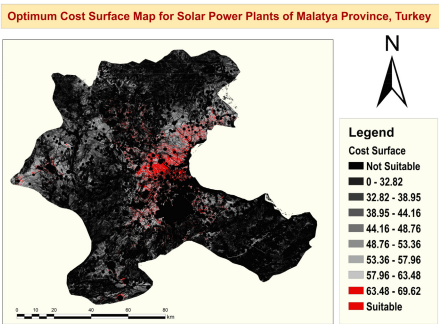
\includegraphics[width=0.5\textwidth]{Figures/Colak.png} % Adjust the width as needed
		\caption{Suitable sites for Solar Powerplant wiht cost factor by author Colak et al.\cite{colak2020}}
		\label{fig:my_label} % Use this label to reference the figure elsewhere
	\end{figure}

	A similar study was conducted by Al Garni et al. in Saudi Arabia\cite{garni2017}. The available land was categorized into five classes: least suitable, marginally suitable, 
	moderately suitable, highly suitable, and most suitable. The decision-making process for site selection unfolded in three phases:
	\begin{enumerate}
		\item Setting decision criteria and restrictions for the site selection study.
		\item Prioritizing sites with high solar potential.
		\item Conducting an analysis on the prioritized regions for informed decision-making.
	\end{enumerate}

	Like the aforementioned study, the authors relied on GIS data provided by NREL, selecting attributes that determined the criteria for site selection. 
	These included DEM, Solar irradiation, and Air Temperature. Broadly, these factors can be divided into two categories: technical (factors affecting energy production) 
	and economical (factors influencing the economic viability of the project).

	Zoghi et al. proposed dividing the factors into four major categories for their case study carried out in Isfahan province, Iran\cite{zoghi2017}:
	\begin{enumerate}
		\item \textbf{Environmental:} Land use, Protected Areas, Wetlands, and Water Resource.
		\item \textbf{Geomorphological:} Elevation, Slope, and Aspect.
		\item \textbf{Location:} Distance to City, Distance to Power line, and Distance to Transport network.
		\item \textbf{Climatic:} Sunshine, Cloudy Days, Dusty Days, Solar Radiation, Rainy and Snowy Days, and Humidity.
	\end{enumerate}

	The study carried out by Saraswat et al. (2021) represents the most elaborate case study for site selection of solar \ac{PV} plants in India, 
	to the best of the student's knowledge\cite{saraswat2021}. A significant limitation of this study is the data's spatial resolution. With a resolution of 
	around 1000m, it is not well-suited for detailed DEM modeling and other attributes. Consequently, the solar farm suitability map produced in this study lacks
	 granularity at a spatial level. However, various databases, provided by USGS and \ac{NREL}, offer spatial resolutions of 30m and can be employed to yield more accurate predictions.

	Data for the study were sourced from multiple governmental bodies: \ac{NREL} for solar radiation, DIVA-GIS for roads and inland water bodies, and the DEM model was provided by the United States Geological Survey (USGS). The factors were segmented into three categories: technical, socio-environmental, and economic.
	\begin{enumerate}
		\item \textbf{Technical:} Solar Radiation, Slope, Aspect, and Elevation.
		\item \textbf{Socio-Environmental:} Distance from coastline, Distance from water bodies, airports, and Land use.
		\item \textbf{Economic:} Distance from urban areas, roads, transmission lines, and power plants.
	\end{enumerate}

	\section{Data Sources and Overview}

	For this project, we required multiple layers of GIS data that would serve as essential features for identifying suitable locations for solar farms. 
	Terrain information is a pivotal feature for this study. To set up a solar farm, vast expanses of land with minimal elevation changes are necessary. 
	Another critical attribute is solar irradiance, which is defined as the power potential generated from solar radiation incident on a specific location, 
	measured in watts per square meter (W/m\textsuperscript{2}). Additional crucial factors to consider include land cost, population density, land use, and 
	protected wildlife sanctuaries.

	\begin{figure}[H]
		\centering
		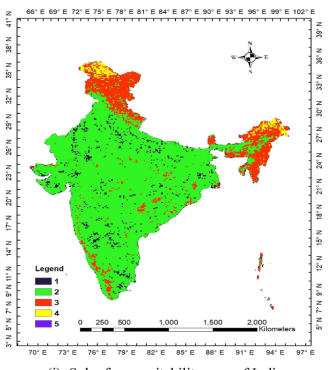
\includegraphics[width=0.5\textwidth]{Figures/Saraswat.png} % Adjust the width as needed
		\caption{ Optimal sites by level of importance by author \cite{saraswat2021}}
		\label{fig:my_label} % Use this label to reference the figure elsewhere
	\end{figure}
	

	\subsection{Terrain Data}

	The \ac{USGS}) is an agency of the United States government that operates across disciplines such as geology, geography, and hydrology. 
	The \ac{SRTM} was undertaken in collaboration with \ac{NASA} to create \ac{DEM} 
	of the earth's surface. This effort produced two Digital Elevation Models available for research, with spatial resolutions of 1 arc-second (30 meters) and 3 arc-second 
	(90 meters). For this study, we will be using the DEM model with a 1 arc-second spatial resolution\cite{farr2000}.

	\begin{figure}[H]
		\centering
		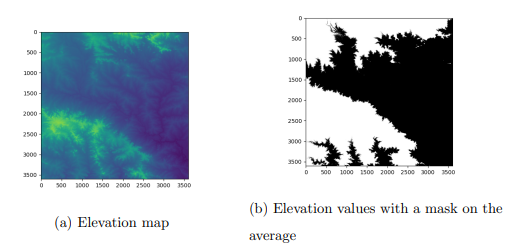
\includegraphics[width=0.8\textwidth]{Figures/Terrain.png} % Adjust the width as needed
		\caption{Elevation map for coordinates N 20' E 78}
		\label{fig:my_label2} % Use this label to reference the figure elsewhere
	\end{figure}

	\subsection{ Solar Irradiance Data}

	The \ac{NSRDB} provides a comprehensive collection of solar irradiance data. This database, which is calculated on both hourly and 
	half-hourly bases, is maintained by the \ac{NREL}, the U.S. Department of Energy, and various other contributors\cite{sengupta2018}. 

	Solar irradiance is characterized by three distinct measurements:

	\begin{itemize}
		\item \textbf{\ac{GHI}:} This refers to the total amount of solar radiation received per unit area on the Earth's surface. It is a cumulative measure that encompasses diffuse horizontal irradiance, ground-reflected radiation, and diffuse sky radiation.
		
		\item \textbf{\ac{DNI}:} \ac{DNI} indicates the amount of solar radiation received per unit area on a surface that is perpendicular to the sun rays incident on that surface.
		
		\item \textbf{\ac{DHI}:} This measurement pertains to the solar radiation that is scattered from the sky, excluding the direct solar beam.
	\end{itemize}

	\begin{figure}[H]
		\centering
		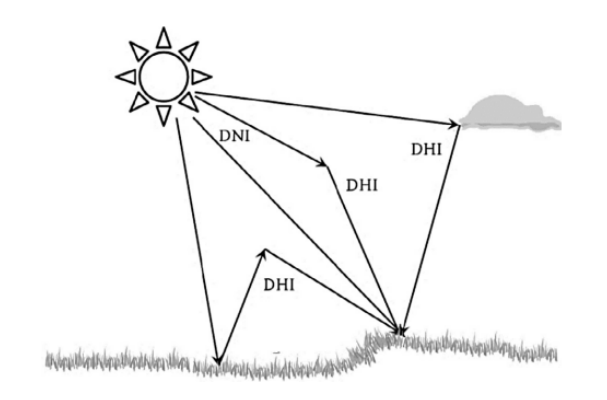
\includegraphics[width=0.5\textwidth]{Figures/Solar Irradiance.png} % Adjust the width as needed
		\caption{Solar Irradiance components\cite{vignola2023}}
		\label{fig:my_label3} % Use this label to reference the figure elsewhere
	\end{figure}


	\begin{figure}[H]
		\centering
		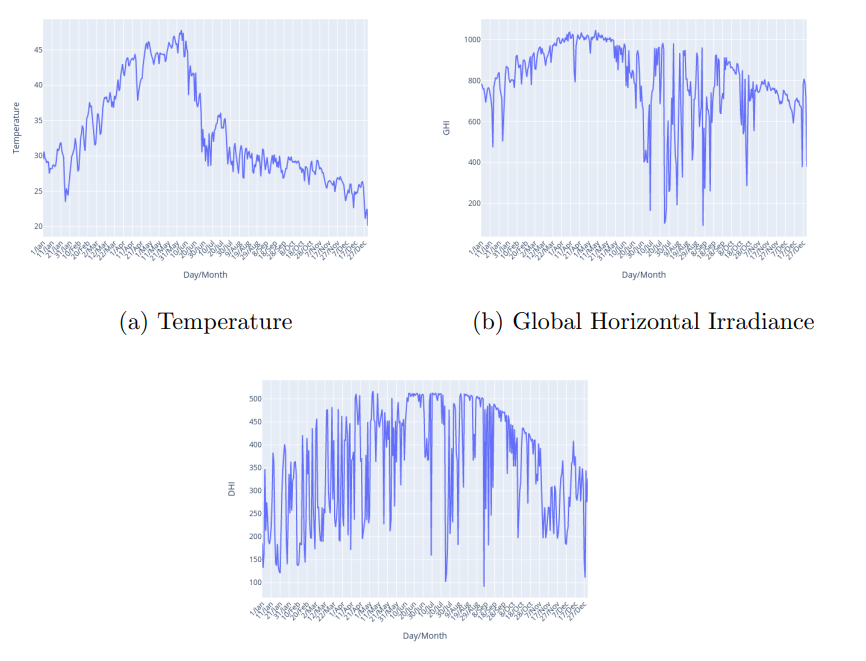
\includegraphics[width=1\textwidth]{Figures/Solar Graphs.png} % Adjust the width as needed
		\caption{Solar irradiance data for co-ordinates for coordinates N 20' E 78'}
		\label{fig:my_label4} % Use this label to reference the figure elsewhere
	\end{figure}

	\subsection{Other Important Attributes}

	While solar irradiance and elevation are critical features to consider when planning the setup of a solar farm, there are numerous other factors that warrant attention. 
	These include:

	\begin{itemize}
		\item \textbf{Financial Viability:} It's essential to assess whether there's sufficient demand for energy in the region to sustain a solar farm.
		
		\item \textbf{Environmental Impact:} Careful consideration must be given to the potential environmental repercussions of developing a solar plant, especially in ecologically sensitive regions.
		
		\item \textbf{Land-use Guidelines:} The designated or allowable uses of a land parcel can influence its suitability for solar farming.
		
		\item \textbf{Skilled Labor:} The availability of trained professionals and workers in the vicinity can have a bearing on the feasibility of the project.
	\end{itemize}

	\ac{OSM} is an open-source collaborative project initiated in 2004, with the objective of creating free geographic data. Over the years, 
	it has evolved into a global community-driven initiative. The maps and data generated by OSM collaborators can be leveraged for various attributes required 
	for such projects~\cite{openstreetmap2017}.
	\begin{figure}[H]
		\centering
		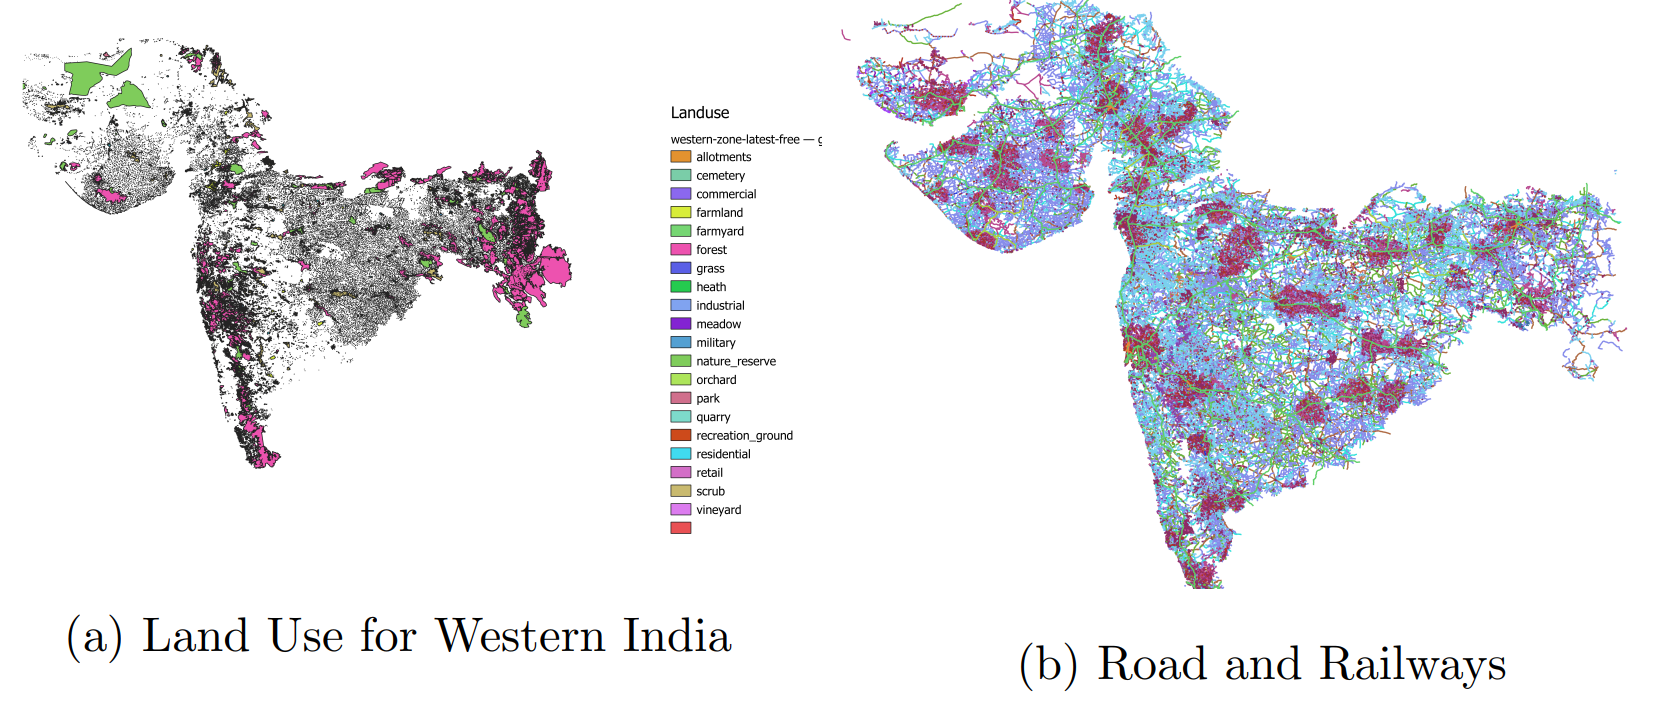
\includegraphics[width=1\textwidth]{Figures/Other attributes.png} % Adjust the width as needed
		\caption{Attributes for Western India}
		\label{fig:my_label5} % Use this label to reference the figure elsewhere
	\end{figure}

	\section{Analytical Hierarchical Process}

	\ac{MCDMs} have been extensively employed in literature for identifying optimal solar PV plant sites. 
	Unlike machine learning techniques, which automatically learn biases without being explicitly programmed, \ac{MCDMs} primarily focus on decision-making based on predefined criteria. 
	These criteria are often ranked manually to guide decision-making processes.

	\ac{AHP} is a widely recognized \ac{MCDMs} technique, as attested by numerous literary sources\cite{colak2020,saraswat2021,garni2017,zoghi2017}. 
	\ac{AHP} was pioneered by Prof. Thomas Saaty\cite{saaty1988}. At its core, \ac{AHP} emphasizes ranking criteria that influence the decision-making process. 

	The methodology of \ac{AHP} can be distilled into three stages:

	\begin{enumerate}
		\item \textbf{Problem Definition and Hierarchy Creation:} Begin by clearly outlining the problem. For the context of this study, the objective is to assess the suitability of a location for a solar PV plant. A hierarchy is then defined based on relevant criteria or factors, which in this instance might encompass aspects like elevation, slope, solar irradiance, land use, and land value.
		
		\item \textbf{Sub-Criteria Classification:} The primary criteria can be further segmented into sub-criteria, enhancing the granularity of the hierarchical structure.
		
		% Add the third stage if there is more information or continue as needed.
	\end{enumerate}

	After establishing a hierarchy, it is essential to define the importance of criteria or factors relative to one another. This can be achieved using a technique known as 
	pairwise comparison. This method involves comparing each factor with every other criterion, and the results of these comparisons can be stored in a matrix, termed the 
	pairwise comparison matrix.

	Once each factor's pairwise comparison with others is documented, the subsequent step is to determine the weights for each criterion. To do this, the matrix is first normalized. 
	Subsequently, a weighted sum of the normalized criteria weights is computed to produce a score. From the normalized vector values, the Consistency Ratio (CR) is determined to 
	validate the hierarchy's legitimacy.

	The Consistency Ratio is a crucial metric that underpins the reliability of the decision-making process. A Consistency Ratio below \(0.1\) suggests that the weights generated 
	can be deemed consistent and acceptable~\cite{saaty1988}.

	The Consistency Ratio (CR), Consistency Index (CI), and Random Consistency Index (RI) are interconnected. The formula to determine CR is:
	\[ CR = \frac{CI}{RI} \]

	Here, RI serves as a reference value instrumental in gauging the consistency of pairwise comparisons. It offers a benchmark for verifying the attained consistency for the pre-defined hierarchy. Meanwhile, CI is derived from the eigenvalue of the pairwise comparison matrix, and it is given by:
	\[ CI = \frac{\lambda_{\text{max}} - n}{n - 1} \]
	Where \(n\) represents the number of criteria under consideration, and \(\lambda_{\text{max}}\) is the largest eigenvalue.


	\section{Kohonen's Model}

	The Kohonen model, also known as the Kohonen neural network or \ac{SOM}, is an unsupervised clustering algorithm. It was introduced by Kohonen et al. 
	in 1982\cite{kohonen1982}. Typically, it is employed for clustering tasks. Notably, Chang et al. utilized it extensively to identify locations with high landslide susceptibility
	\cite{chang2020}.

	One of the primary objectives of the Kohonen model is dimensionality reduction. The aim is to generate a low-dimensional representation while retaining the inherent 
	properties of the data. This is accomplished by associating each neuron with a weight vector that has the same dimension as the input data. These weights are iteratively 
	aligned to match the distribution of the input data.

	Initially, all the weight vectors of the neurons are initialized with random values drawn from a normal distribution. Iteratively, input vectors are selected from the 
	training data. To compute the proximity of the input vector to the weighted vector, a distance or similarity metric, such as the Euclidean distance or cosine similarity, 
	is employed. The \ac{BMU} is the neuron whose weight vector most closely matches the input vector. Subsequently, the weights of the neurons are updated to 
	align more closely with the selected input vector. This process continues iteratively until convergence.

	Upon completion of the training phase, the Kohonen model produces a lower-dimensional vector space representation of the input data. The number of neurons in the model 
	signifies the number of classes or clusters intended for classification. It's worth noting that the Kohonen model can be supplied with vectorized GIS data spanning multiple 
	criteria, as demonstrated by Chang et al. in their research on landslide susceptibility\cite{chang2020}.

	\section{Auto Encoder and Multi-Layer Perceptron}

	Ahmadlou et al. conducted comprehensive research on flood susceptibility in both Iran and India~\cite{ahmadlou2020}. In their study, geospatial data, including layers such as 
	slope, aspect, altitude, land use, and rainfall, served as determining criteria for the model~\cite{ahmadlou2020}.

	\begin{figure}[H]
		\centering
		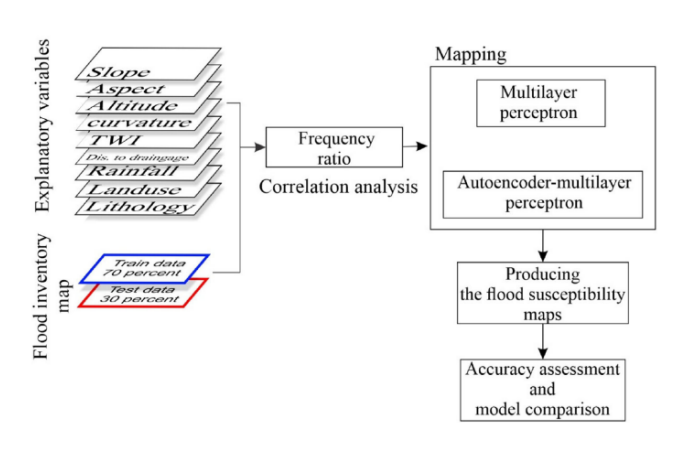
\includegraphics[width=1\textwidth]{Figures/AutoEncoder.png} % Adjust the width as needed
		\caption{Flowchart of the model proposed by\cite{ahmadlou2020}}
		\label{fig:my_label8} % Use this label to reference the figure elsewhere
	\end{figure}

	They employed a hybrid model combining a \ac{MLP} and an Auto-Encoder. The Auto-Encoder is a type of neural network architecture proposed by 
	Hinton and Rumelhart~\cite{rumelhart1986}. It comprises an encoder and a decoder, which collaboratively work to diminish the dimensionality of the input vector, 
	representing it in a more condensed vector space known as the latent space. In this setup, the Auto-Encoder functions primarily as a feature extractor. 
	The extracted features are subsequently used to train an \ac{MLP} for making predictions.

	An auto-encoder essentially operates as a neural network aiming to recreate its input. Structurally, it is segmented into three main components:

	\begin{enumerate}
		\item \textbf{Encoder:} It compresses the data into a lower-dimensional vector space. The encoder uses a neural network with transformational layers such as fully connected,
		 convolutional, and dropout layers.
		
		\item \textbf{Latent Space:} This represents the compressed version of the input vector produced by the encoder. Serving as a bottleneck, it retains the core features of
		 the data.
		
		\item \textbf{Decoder:} This component of the neural network endeavors to reconstruct the original input vector. Its primary function lies in computing 
		the reconstruction cost.
	\end{enumerate}

	During the training process of an auto-encoder, the decoder's output is juxtaposed with the original input. The discrepancy in the reconstructed output is termed as the reconstruction error. 
	This error is minimized using the backpropagation algorithm until convergence is achieved. Once trained, the encoder can then be utilized to produce a lower-dimensional 
	representation of the data, which can be harnessed for various machine learning tasks.

	\chapter{Methodology}
	\label{chap:methodology}

	For the task at hand, a novel methodology is proposed in this project. The features considered for this task, as mentioned in Section 2.2[Data Sources and Overview], 
	can be subdivided into three classes:

	\begin{enumerate}
		\item \textbf{Terrain Information:} In this case, the elevation model, denoted by \ac{DEM}, was readily available from the \ac{SRTM} mission undertaken by \ac{USGS}. This data, with a spatial resolution of 30m, is superior to the data used in previous studies by other authors. Additionally, the slope of the terrain is another crucial factor. The slope determines the amount of solar irradiance incident on the surface of the \ac{PV} cells. Furthermore, a steep slope would not be suitable for a solar \ac{PV} farm.
		
		\item \textbf{Solar Irradiance and Atmospheric Conditions:} These were sourced from \ac{NREL}. They play a pivotal role in identifying suitable locations. Specifically, a region with high solar irradiance, minimal overcast conditions, and high temperatures would be ideal.
		
		\item \textbf{Other Features:} For this project, we also considered \ac{GIS} layers from the \ac{OSM} dataset. This includes features such as railways, roadways, land use, landmarks, and urban areas.
	\end{enumerate}
	
	The primary objective here is to employ K-means clustering to create clusters and identify the most suitable ones based on locations that already contain a solar PV plant within the appropriate cluster. 
	However, given the data's diversity and high dimensionality, it's essential to reduce its dimensionality and integrate our data from various sources before applying the clustering techniques.

	\section{Data Cleaning and Preprocessing}

	\section{Data Modelling}

	\section{Algorithm}
	\subsection{AutoEncoder}
	\subsection{Clustering}

	
	\chapter{Experiments}

	\section{Experiments}
	\section{Results}

	\chapter{Conclusion}
	\label{chap:conclusion}
	\section{Future Scope}
	\section{Conclusion}

	
	Here you must zoom back out to evaluate the thesis. Mention limitations and weaknesses as well as contributions and possible future work.
	
	%%%%%%%%%%%%%%%%%%%%%%%%%%%%%%%%%%%%%%%%%%%%%%%%%%%%%%%%%%%%%%%%%%%%%%%%%%%%%%%%
	%\bibliographystyle{plainnat}                  % to give author-year style
	\bibliographystyle{IEEEtranN} 
	\renewcommand{\bibname}{References}           % change default name Bibliography to References
	\bibliography{references}                     % BibTeX References file, references.bib
	\addcontentsline{toc}{chapter}{References}    % add References to TOC
	
	
	%%% uncomment if Appendix needed
	%\appendix
	%\chapter{Appendix-A-Title} 
	%\label{chap:appendix_a}
	
	%\chapter{Appendix-B-Title} 
	%\label{chap:appendix_b}
	
\end{document}
